
\clearpage

\section{Modificaciones PDB4DNA}
\label{sec:MODIFI}
PDB4DNA fue modificado de tal manera que en vez de hacer uso de las esferas ligadas a partir de barycentros usara centros de masa, para esto se uso el archivo PDBlib, primero se definió la masa de los diferentes elementos (véase anexo ~\ref{app:A}),y luego se usaron las clases bases ya definidas en PDBlib para hacer los respectivos cálculos de centros de masa(véase anexo ~\ref{app:B}).\\
Al graficar con Geant4 no se observa ningún cambio drástico


\begin{figure}
\centering
\begin{subfigure}{.6\textwidth}
  \centering
  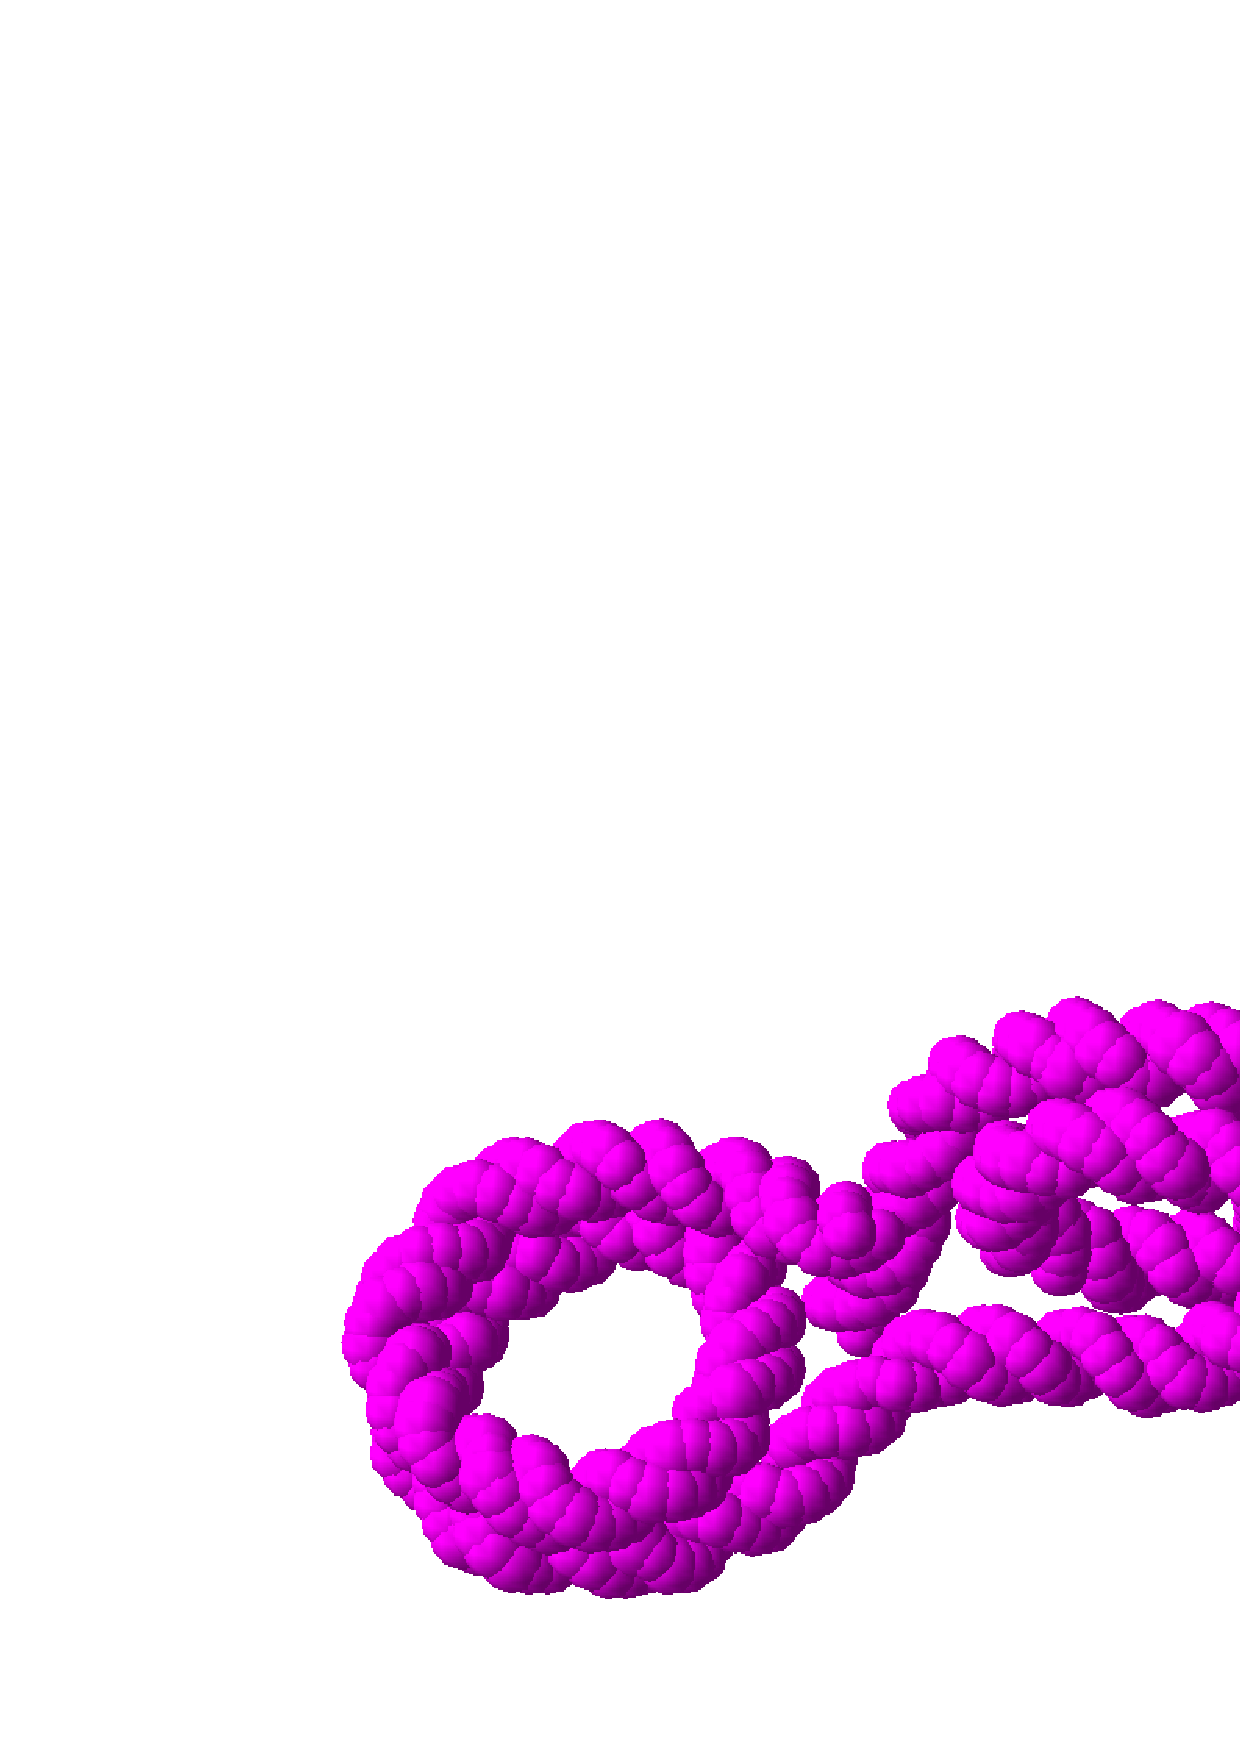
\includegraphics[width=.7\linewidth]{./Figures/a.png}
  \caption{Barycentros}
  \label{fig:sub1}
\end{subfigure}%
\begin{subfigure}{.5\textwidth}
  \centering
  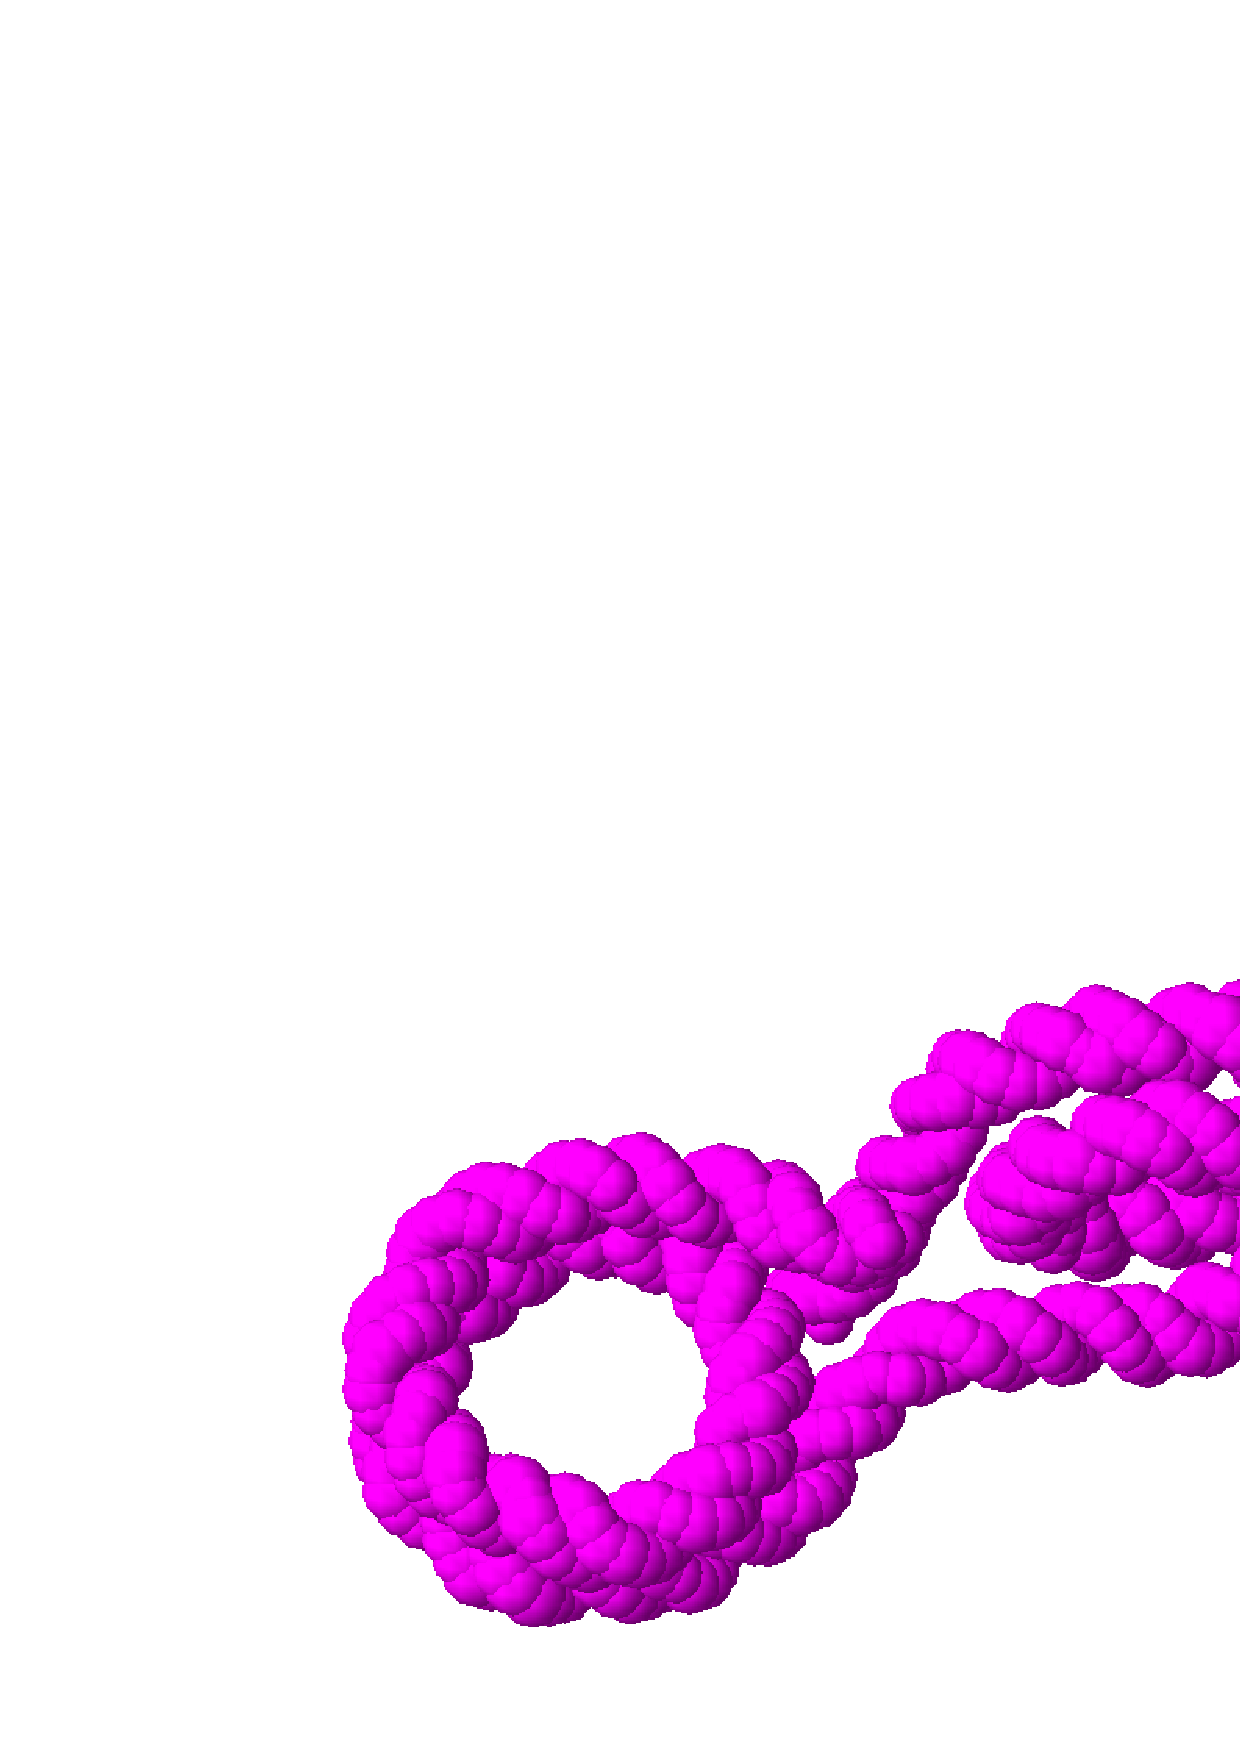
\includegraphics[width=.7\linewidth]{./Figures/b.png}
  \caption{Centros de masa}
  \label{fig:sub2}
\end{subfigure}
\caption{Comparación barycentros y centros de masa en Geant4}
\label{fig:test}
\end{figure}


\begin{figure}[htbp]
    \centering
    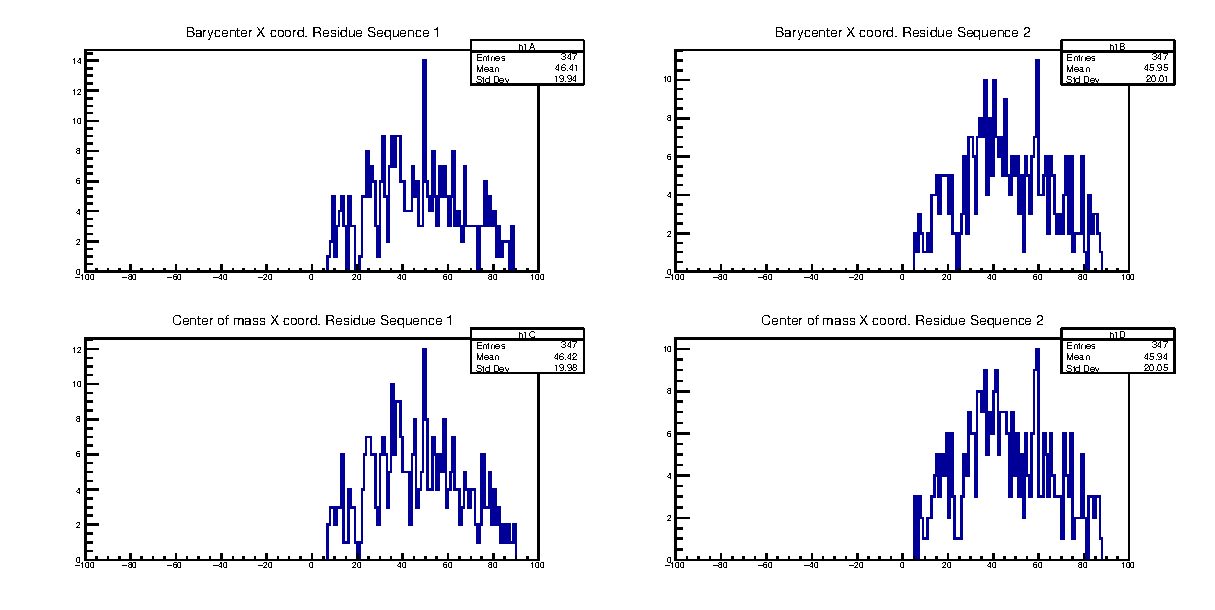
\includegraphics[width=1\linewidth]{./Figures/can1.eps}
    \caption[Barycentros vs centros de masa en x]{Barycentros vs centros de masa en x} % se puede realizar grafico en vmd}
    \label{fig:canx}
\end{figure}

\begin{figure}[htbp]
    \centering
    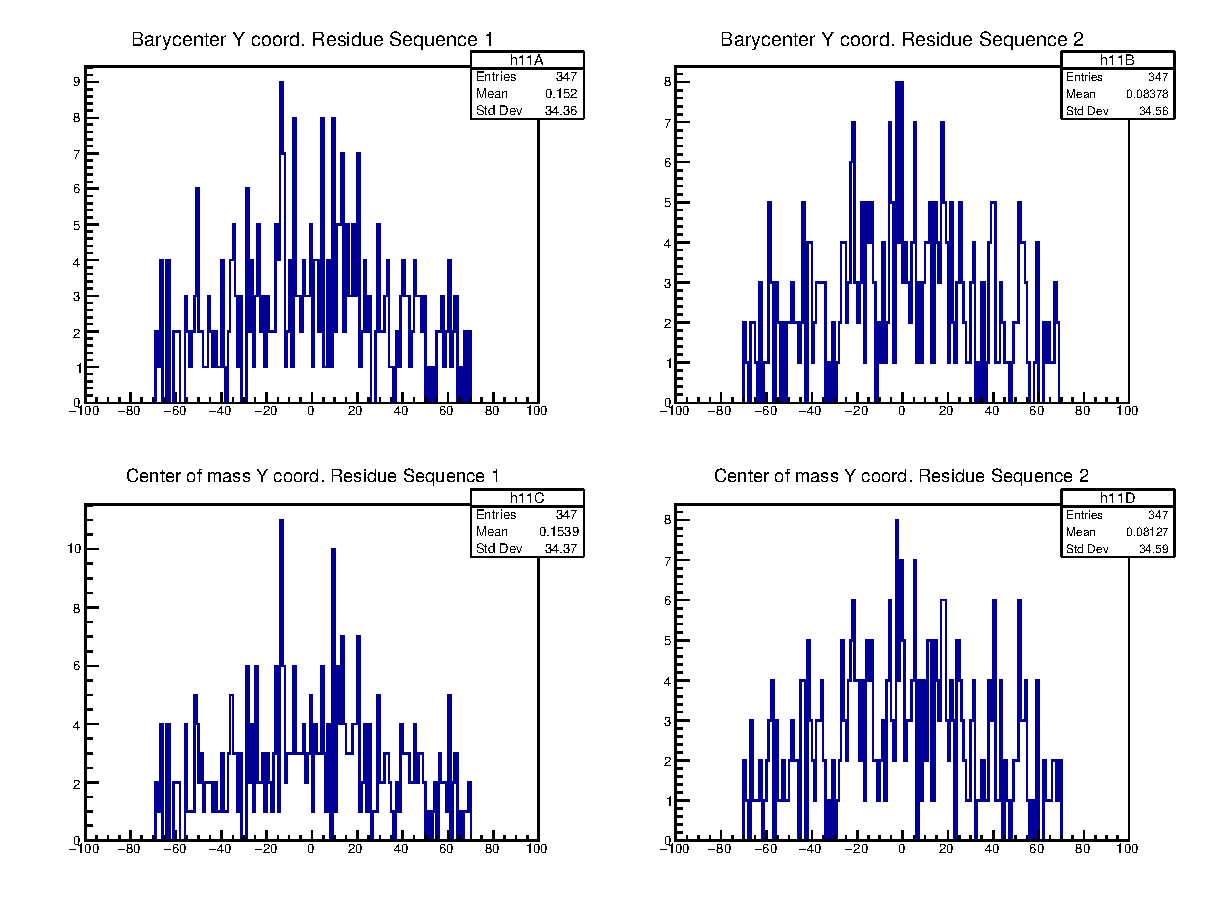
\includegraphics[width=1\linewidth]{./Figures/can2.eps}
    \caption[Barycentros vs centros de masa en y]{Barycentros vs centros de masa en y}
    \label{fig:cany}
\end{figure}

\begin{figure}[htbp]
    \centering
    \includegraphics[width=1\linewidth]{./Figures/can3.eps}
  \caption[Barycentros vs centros de masa en z]{Barycentros vs centros de masa en z}
    \label{fig:canz}
\end{figure}
